\chapter{Basics of Sweet.JS}

Sweet.js implements macros for JavaScript, which takes source code written with Sweet.JS macros and produces the expanded source that can be run in any JavaScript environment. 
\section{Type of macros in Sweet.JS}
\begin{enumerate}
\item {\bf Rule macros }
Rule macros work by matching a syntax pattern and generating new syntax based on the template.
To define a rule base macro the grammar is
\begin{lstlisting}[frame=single]
macro <name> {
  rule { <pattern> } => { <template> }
}
\end{lstlisting} 

The following macro defines swapping of two number
\begin{lstlisting}[frame=single]
	macro swap {
    	rule { ($x, $y) } => {
        	var tmp = $x;
        	$x = $y;
        	$y = tmp;
    	}
	}
	var foo = 5;
	var tmp = 6;
	swap(foo, tmp);
\end{lstlisting} 

When the compiler hits "swap", it invokes the macro and runs each rule against the code after it. When a pattern is matched, it returns the code within the rule. You can bind identifiers \& expressions within the matching pattern and use them within the code.

if Sweet.js did not support hygiene, this macro might expand to
\begin{lstlisting}[frame=single]
	var foo = 5;
	var tmp = 6;
	var tmp = foo;
	foo = tmp;
	tmp = tmp;
\end{lstlisting} 
The \texttt{tmp} created from the macro collides with my local \texttt{tmp}. This is a serious problem, but macros solve this by implementing hygiene. Basically they track the scope of variables during expansion and rename them to maintain the correct scope. Sweet.js fully implements hygiene so it never generates the code you see above. It would actually generate the following code
\begin{lstlisting}[frame=single]
	var foo = 5;
	var tmp$1 = 6;
	var tmp$2 = foo;
	foo = tmp$1;
	tmp$1 = tmp$2;
\end{lstlisting} 
Notice how two different "tmp" variables are created. This makes it extremely powerful to create complex macros elegantly.

\item {\bf Case macros }
Case macro are analogous to syntax-case in Scheme. Case macro allow the macro author to use JavaScript code to procedurally create and manipulate the syntax.
To define case macro, the grammar is
\begin{lstlisting}[frame=single]
	macro <name> {
  		case { <pattern> } => { <body> }
	}
\end{lstlisting}
Example
\begin{lstlisting}[frame=single]
	macro rand {
  	  case { _ $x } => {
    	    var r = Math.random();
     	   letstx $r = [makeValue(r)];
      	 return #{ var $x = $r }
   		}
	}

	rand x;
\end{lstlisting}

The above code expand to

\begin{lstlisting}[frame=single]
	var x$123 = 0.8367501533161177;
\end{lstlisting}

The body of a macro contains a mixture of templates and normal JavaScript that can create and manipulate syntax
The code within the ``case'' is run at expand-time and you use \#\{\} to create "templates" that construct code just like the syntax in the rule macros.

\end{enumerate}

\section{How Sweet.JS work?}

The JavaScript macro system, Sweet.JS includes a separate reader that converts a sequence of tokens into a sequence of token trees, Analogous to s-expressions in scheme,without feedback from the parser.

\begin{figure}[htb]
\centering
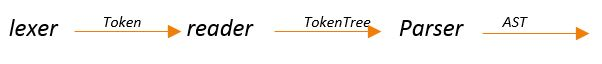
\includegraphics[width=0.8\textwidth]{images/Tokenizer.jpg}
\caption{Sweet.JS anatomy.} 
\label{fig:Tokenizer}
\end{figure}

The parser gives structure to unstructured source code. The lexer which converts a character stream to a token stream and a parser converts the token stream into an AST according to a context free grammar ~\cite{bib2}.The macro expander  must sit in between the lexer and the parser.Here the reader records sufficiently history information in the form of token trees in order to decide how to parse the token, which is required to decide if token is a divisor or a regular expression.
In traditional JavaScript compilers, the parser and lexer are intertwined, rather than run the entire program through the lexer once to get a sequence of tokens, the parser calls out to the lexer from a given grammatical context with a flag to indicate if the lexer should accept a regular expression or a divide operator and the input character are tokenized accordingly ~\cite{bib2}.

Example

\begin{lstlisting}[frame=single]
	macro id {
  		case {_ $x } => {
   			return #{ $x }
  		}
	}
	id 42
\end{lstlisting}
\newpage
\begin{figure}[htb]
\centering
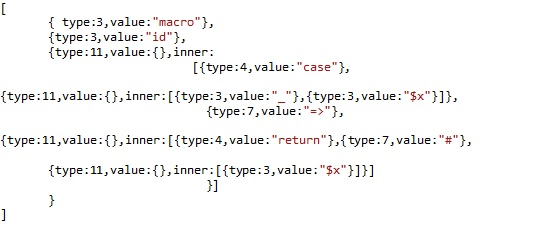
\includegraphics[width=1.0\textwidth]{images/readeroutput.jpg}
\caption{Token tree.} 
\label{fig:readeroutput}
\end{figure}
Reader convert string of token to token tree, 
\begin{figure}[htb]
\centering
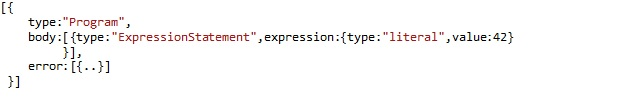
\includegraphics[width=1.0\textwidth]{images/AST.jpg}
\caption{Final AST from parser.} 
\label{fig:AST}

\end{figure}

Parser give structure to unstructured source code, In parsers without macro systems this is usually accomplished by a lexer which convert a character stream to a token stream and a parser which convert the token stream into an AST according to a context-free grammar.

The approach used in Sweet.JS is \textit{Enforestation},first pioneered by Honu ~\cite{bib4}. Enforestation means transformation,extracts the sequence of terms produced by the reader to create a term tree. Consider following let example

\begin{figure}[htb]
\centering
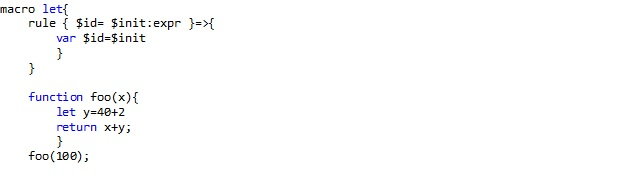
\includegraphics[width=1.0\textwidth]{images/enforest.jpg}
\caption{Macro Expansion.} 
\label{fig:AST}

\end{figure}
Enforestation begins by loading the let macro into the macro environment and converting the function declaration into a term tree.

\begin{figure}[htb]
\centering
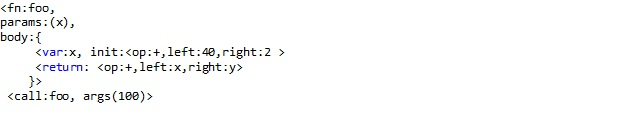
\includegraphics[width=1.0\textwidth]{images/enforest1.jpg}
\caption{Term tree.} 
\label{fig:AST}

\end{figure}

A term tree is a kind of proto-AST that represent a partial parse of the program. As the expander passes through the token trees, it creates term trees that contain unexpanded sub trees that will be expanded once all macro definition have been discovered in the current scope.

\section{Problem trying to solve?}

Although the benefits of hygienic macros are well established, there are occasions when traditional hygienic bindings are insufficient. The classic example is "anaphoric conditionals" where the value of the tested expression is available as an \textsc{it} bindings.When the condition is true, an \textsc{it} identifier is automatically created and set to the value of the condition. An anaphoric macro is a type of programming macro that deliberately captures some form supplied to the macro which may be referred to by an anaphor (an expression referring to another).

\newpage
\begin{figure}
\centering
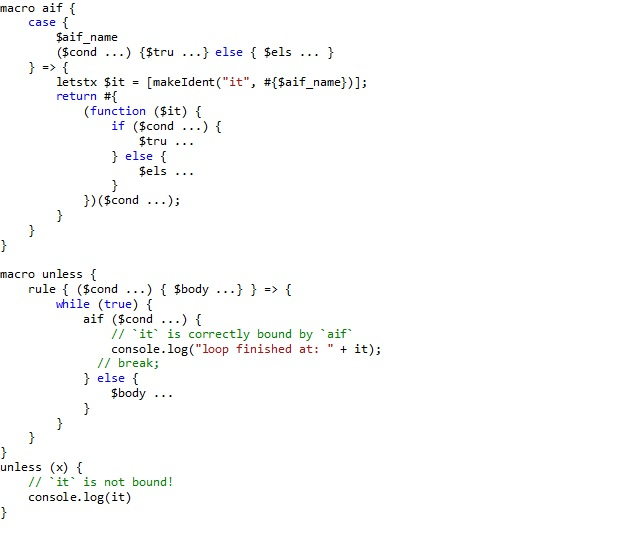
\includegraphics[width=1.0\textwidth]{images/Breakhygiene.jpg}
\caption{Break hygienic in Sweet.JS.} 
\label{fig:Breakhygiene}

\end{figure}
In above example, I define "unless" macro which run until condition is met, which in turn call the anaphoric-if condition which introduces an anaphor \textsc{it} which should bound to the result of the test clause.

\newpage
\begin{figure}

\centering
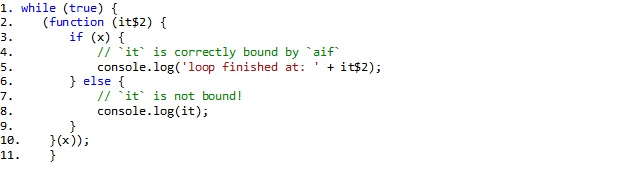
\includegraphics[width=1.0\textwidth]{images/macroexpansion.jpg}
\caption{Macro expansion.} 
\label{fig:macroexpansion}

\end{figure}

\newpage

In above macro expansion [Figure 7], at line (8) identifier \textsc{it} is not defined. Here we wish to introduce the identifiers deliberately breaking hygiene. 

Same unhygienic macros are possible in Scheme as shown in the below example, mistake is if our new syntax introduces a variable that conflicts with one in the code surrounding our macro.

\begin{lstlisting}[frame=single]
(define-syntax-rule (aif condition true-expr false-expr)
 (let ([it condition])
   (if it
      true-expr
      false-expr)))

 (aif #t (displayln it) (void))

it: undefined;
cannot reference an identifier before its definition
in module: 'program
\end{lstlisting}

When using syntax-parameterize, \textsc{it} acts as an alias for \textsc{tmp}. The alias behavior is created by make-rename-transformer. \textbf{define-syntax-parameter}, binds the keyword to the value obtained by evaluating the transformer. The transformer provides the default expansion for the syntax parameter. \textbf{syntax-parameterize}, adjust the keyword to use the values obtained by evaluating their transformer in the expansion of the expression. 

\begin{lstlisting}[frame=single][frame=single]
(require racket/stxparam)
(define-syntax-parameter it
   (lambda (stx)
   (raise-syntax-error (syntax-e stx)
     "can only be used inside aif")))

(define-syntax-rule (aif condition true-expr false-expr)
   (let ([tmp condition])
   (if tmp
   (syntax-parameterize ([it (make-rename-transformer #'tmp)])
     true-expr)
     false-expr)))
\end{lstlisting}
"define-syntax-parameter," binds keyword to the value obtained by evaluating transformer. The transformer provide the default expansion for the syntax parameter."syntax-parameterize," adjust keyword to use the values obtained by evaluating their transformer in the expansion of the expression. 
